% main.tex
% ECE340 Final Project Report

\documentclass[11pt,a4paper]{article}

\usepackage[margin=1in]{geometry}
\usepackage{amsmath,amssymb,bm}
\usepackage{graphicx}
\usepackage{booktabs}
\usepackage{siunitx}
\usepackage{subcaption}
\usepackage{hyperref}
\usepackage{xcolor}
\usepackage{enumitem}
\usepackage{caption}

\hypersetup{
    colorlinks=true,
    linkcolor=blue,
    citecolor=blue,
    urlcolor=blue
}

\sisetup{
    scientific-notation=true,
    per-mode=symbol
}

\graphicspath{{figures/}}

\title{Verification of Diode Physics Using Driftfusion}
\author{
    \textbf{Simulation Group:} Guo Wangyihan (1A), Yang Chenhan (1B), Jiang Ding (1C) \\
    \textbf{Theory Group:} Ma Yinfei (2A), Wang Jiachang (2B), Ji Yaofang (2C) \\
    \textbf{Report Group:} Chen Zhenbo (3A), Shen Yishan (3B), Liu Yuxuan (3C) \\
    ECE340: Semiconductor Devices
}
\date{Spring 2026}

\newcommand{\jzero}{J_0}
\newcommand{\jsc}{J_{SC}}
\newcommand{\voc}{V_{OC}}
\newcommand{\vbi}{V_{bi}}
\newcommand{\Na}{N_A}
\newcommand{\Nd}{N_D}
\newcommand{\di}{d_i}
\newcommand{\um}{\si{\micro\meter}}

\begin{document}

\maketitle

\begin{abstract}
This project uses the Driftfusion one-dimensional drift-diffusion simulator to verify standard diode physics for silicon p--n junctions and PIN diodes, with particular attention to where textbook analytical models remain accurate and where they begin to miss non-ideal effects. The numerical workflow consists of equilibrium simulation, dark current-voltage sweeps, and illuminated current-voltage sweeps. From these simulations, the built-in potential $\vbi$, depletion width $W$, saturation current density $\jzero$, short-circuit current density $\jsc$, and open-circuit voltage $\voc$ are extracted and compared with analytical diode models. The equilibrium electrostatic quantities agree well with analytical formulas, showing that Poisson/depletion theory captures the junction electrostatics robustly. In contrast, current-related quantities such as $\jzero$ are more sensitive to finite device thickness, surface recombination, SRH recombination, and numerical extraction criteria. PIN diode simulations show that increasing the intrinsic-layer thickness increases generation volume and widens the depleted region, supporting drift-based carrier collection. Overall, the deviations are the most informative part of the comparison because they show which quantities are robustly captured by simple formulas and which require numerical drift-diffusion simulation.
\end{abstract}

\tableofcontents
\newpage

\section{Introduction}

\subsection{Background and Project Goals}

p--n junctions and PIN diodes are fundamental semiconductor devices. A p--n junction demonstrates rectification, depletion-region formation, built-in potential, and minority-carrier injection. A PIN diode extends this structure by inserting a lightly doped or intrinsic layer between the p-type and n-type regions, which widens the depleted region and is especially useful for photodetection and high-frequency carrier collection.

The purpose of this project is not to design a new device. Instead, the goal is to use Driftfusion as a numerical semiconductor-device simulator and compare the simulated results with standard analytical diode equations. The project is organized around three questions:

\begin{enumerate}[leftmargin=2em]
    \item Can a baseline silicon p--n junction reproduce rectifying J--V behavior and the expected values of $\jzero$, $\jsc$, and $\voc$?
    \item How do doping concentrations affect $\vbi$, depletion width $W$, and $\jzero$?
    \item How does the intrinsic-layer thickness in a PIN diode affect photocurrent, depletion width, and carrier-collection behavior?
\end{enumerate}

These questions follow the project guidance: simulate p--n junctions and PIN diodes, extract physically meaningful quantities, and compare numerical results with analytical models.

\subsection{Report Organization}

Section 2 describes the Driftfusion simulation workflow and extraction methods. Section 3 summarizes the analytical formulas used for comparison. Section 4 presents the results for the baseline p--n junction, doping-dependence study, and PIN diode simulations. Section 5 concludes by summarizing the main physical trends and the limitations of the comparison.

\section{Methodology}

\subsection{Driftfusion Simulation Workflow}

Driftfusion is a MATLAB-based drift-diffusion simulation tool for one-dimensional ordered semiconductor devices. It solves carrier continuity equations coupled with Poisson's equation, which makes it suitable for extracting spatial electrostatic quantities such as electric field and potential, as well as terminal J--V characteristics.

The project used three simulation steps:

\begin{itemize}[leftmargin=2em]
    \item \textbf{Equilibrium simulation:} zero-bias equilibrium was used to extract the built-in potential $\vbi$ and the electric-field profile. The depletion width $W$ was estimated from the electric-field profile.
    \item \textbf{Dark J--V sweep:} voltage was swept without optical generation. The semi-log forward-bias region was used to extract the saturation current density $\jzero$.
    \item \textbf{Illuminated J--V sweep:} a uniform optical generation rate was applied. The short-circuit current density $\jsc$ was extracted at $V=0$, and the open-circuit voltage $\voc$ was extracted at $J=0$.
\end{itemize}

\subsection{Baseline p--n Junction Protocol}

The baseline device is a silicon p--n junction with symmetric doping,
\[
    \Na=\Nd=10^{16}\ \si{cm^{-3}}.
\]
The main material and transport parameters are summarized in Table~\ref{tab:baseline_parameters}. The analytical calculations use $n_i=10^{10}\ \si{cm^{-3}}$ at \SI{300}{K}.

\begin{table}[htbp]
    \centering
    \caption{Baseline silicon parameters used for analytical comparison.}
    \label{tab:baseline_parameters}
    \begin{tabular}{ll}
        \toprule
        Parameter & Value \\
        \midrule
        Band gap $E_g$ & \SI{1.12}{eV} \\
        Relative permittivity $\varepsilon_r$ & 11.7 \\
        Electron mobility $\mu_n$ & \SI{1400}{cm^2/(V.s)} \\
        Hole mobility $\mu_p$ & \SI{450}{cm^2/(V.s)} \\
        SRH lifetimes $\tau_n,\tau_p$ & \SI{1e-6}{s} \\
        Intrinsic carrier concentration $n_i$ & \SI{1e10}{cm^{-3}} \\
        Uniform optical generation $g_0$ & \SI{1e21}{cm^{-3}.s^{-1}} \\
        \bottomrule
    \end{tabular}
\end{table}

\subsection{Extraction Methods}

For $\jzero$, the dark current density was plotted as $\ln |J|$ versus voltage. The low-forward-bias region may be affected by depletion-region SRH recombination, while the high-forward-bias region may be affected by series resistance. Therefore, $\jzero$ was extracted from the intermediate forward-bias region, approximately \SIrange{0.2}{0.5}{V}, by fitting the linear semi-log behavior and extrapolating to $V=0$.

For the depletion width, the simulated electric field does not drop abruptly to zero. A practical criterion was used: the depletion edges were taken as the positions where the electric-field magnitude drops to approximately 5\% of its peak value. The distance between these two points was reported as $W$.

\subsection{PIN Diode Protocol}

The PIN diode consists of a p-type silicon layer, a lightly doped intrinsic region, and an n-type silicon layer. The p and n regions use doping near $10^{16}\ \si{cm^{-3}}$, while the intrinsic region is much more lightly doped, approximately $10^{12}\ \si{cm^{-3}}$. The intrinsic-layer thickness was swept over
\[
    \di = 0.5,\ 1,\ 2,\ 5\ \um.
\]
For each thickness, an illuminated J--V simulation was used to extract $|\jsc|$, $\voc$, $W$, and fill factor (FF).

\section{Analytical Models Used for Comparison}

\subsection{Built-in Potential and Depletion Width}

For an abrupt p--n junction at equilibrium, the built-in potential is
\begin{equation}
    \vbi = \frac{kT}{q}\ln\left(\frac{\Na\Nd}{n_i^2}\right).
    \label{eq:vbi}
\end{equation}
For the baseline case with $\Na=\Nd=10^{16}\ \si{cm^{-3}}$ and $n_i=10^{10}\ \si{cm^{-3}}$, this gives
\[
    \vbi \approx \SI{0.714}{V}.
\]

The depletion width under the depletion approximation is
\begin{equation}
    W = \sqrt{\frac{2\varepsilon_s \vbi}{q}\left(\frac{1}{\Na}+\frac{1}{\Nd}\right)},
    \label{eq:depletion_width}
\end{equation}
where $\varepsilon_s=\varepsilon_r\varepsilon_0$. For the baseline case, this gives
\[
    W \approx \SI{0.430}{\um}.
\]

\subsection{Dark Saturation Current Density}

The ideal diffusion-current expression for the saturation current density is
\begin{equation}
    \jzero = \frac{qD_p p_{n0}}{L_p} + \frac{qD_n n_{p0}}{L_n},
    \label{eq:j0}
\end{equation}
where
\begin{equation}
    p_{n0}=\frac{n_i^2}{\Nd}, \qquad n_{p0}=\frac{n_i^2}{\Na}.
    \label{eq:minority_concentration}
\end{equation}
The diffusion coefficients are obtained from the Einstein relation,
\begin{equation}
    D = \mu \frac{kT}{q},
\end{equation}
and the diffusion lengths are
\begin{equation}
    L_n=\sqrt{D_n\tau_n}, \qquad L_p=\sqrt{D_p\tau_p}.
\end{equation}
For the baseline parameters, the analytical value is
\[
    \jzero \approx \SI{1.51e-11}{A/cm^2}.
\]

\subsection{Open-circuit Voltage}

Under illumination, the ideal diode equation gives
\begin{equation}
    \voc = \frac{kT}{q}\ln\left(\frac{|\jsc|}{\jzero}+1\right).
    \label{eq:voc}
\end{equation}
This formula shows that $\voc$ increases with photocurrent and decreases when the saturation current is larger.

\subsection{Asymmetric Junction Approximation}

For a strongly asymmetric $p^+$--$n$ junction, where $\Na \gg \Nd$, the lightly doped n-side dominates the depletion width because $1/\Nd \gg 1/\Na$. Equation~\ref{eq:depletion_width} then becomes approximately
\begin{equation}
    W \approx \sqrt{\frac{2\varepsilon_s \vbi}{q\Nd}}.
\end{equation}
The saturation current is also strongly affected by the minority carrier concentration on the lightly doped side. In this limit, the minority hole current in the n-side can dominate:
\begin{equation}
    \jzero \approx \frac{qD_p n_i^2}{L_p\Nd}.
\end{equation}
This explains why changing the lightly doped side can have a large effect on both $W$ and $\jzero$.

\section{Results and Analysis}

\subsection{Part 1: p--n Junction Verification}

\subsubsection{Dark J--V Characteristics and \texorpdfstring{$\jzero$}{J0} Extraction}

The dark J--V result in Figure~\ref{fig:dark_jv} shows clear rectifying behavior. In forward bias, the current increases approximately exponentially over an intermediate voltage range. This region is used for the $\jzero$ fit because it avoids low-bias recombination curvature and high-bias series-resistance effects.

\begin{figure}[htbp]
    \centering
    \includegraphics[width=0.78\linewidth]{fig1_dark_jv_semilog.pdf}
    \caption{Dark J--V characteristic of the baseline p--n junction. The intermediate forward-bias region is used for extracting $\jzero$.}
    \label{fig:dark_jv}
\end{figure}

\subsubsection{Illuminated J--V, \texorpdfstring{$\jsc$}{JSC}, and \texorpdfstring{$\voc$}{VOC}}

Under uniform optical generation, the illuminated J--V curve shifts downward according to the photogenerated current. As shown in Figure~\ref{fig:illuminated_jv}, $\jsc$ is extracted at zero voltage and $\voc$ is extracted where the current density crosses zero.

\begin{figure}[htbp]
    \centering
    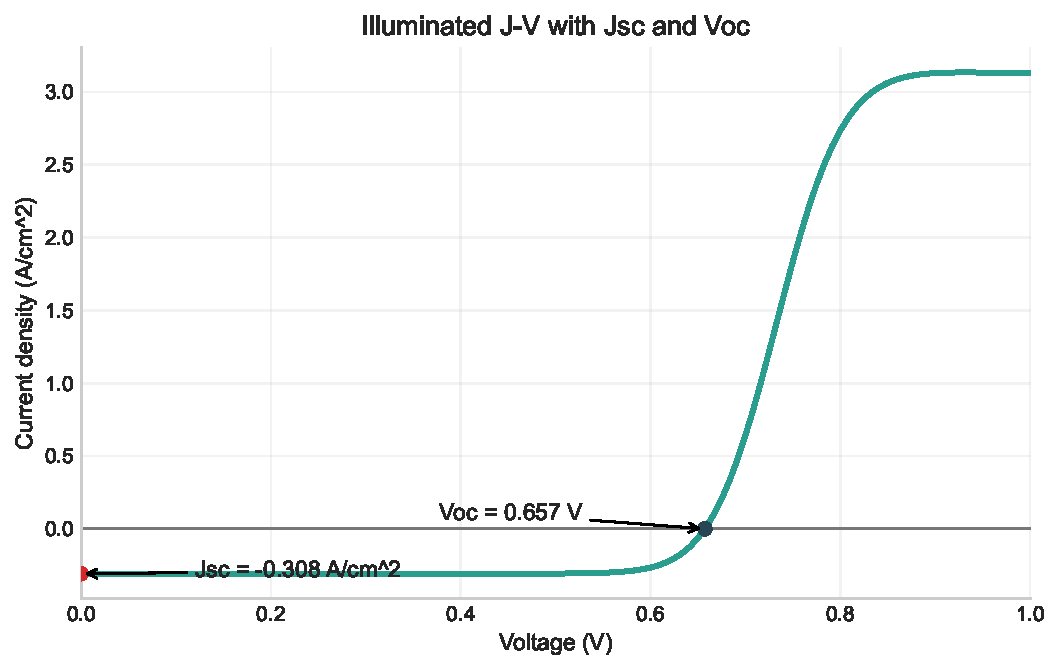
\includegraphics[width=0.78\linewidth]{fig2_illuminated_jv.pdf}
    \caption{Illuminated J--V characteristic under uniform optical generation. $\jsc$ is extracted at $V=0$, and $\voc$ is extracted at $J=0$.}
    \label{fig:illuminated_jv}
\end{figure}

\subsubsection{Comparison with Analytical Theory}

Table~\ref{tab:part1_comparison} compares the baseline analytical values with Driftfusion results. The simulated $\vbi$ is close to the analytical result. The simulated depletion width is larger than the abrupt depletion-approximation value because the electric field decays smoothly, and the 5\% criterion includes part of the Debye tail.

\begin{table}[htbp]
    \centering
    \caption{Baseline p--n junction analytical and simulation comparison.}
    \label{tab:part1_comparison}
    \begin{tabular}{lccc}
        \toprule
        Quantity & Analytical Value & Simulation Value & Difference \\
        \midrule
        $\vbi$ & \SI{0.714}{V} & \SI{0.7352}{V} & +3.0\% \\
        $W$ & \SI{0.430}{\um} & \SI{0.5206}{\um} & +21.1\% \\
        $\jzero$ & \SI{1.51e-11}{A/cm^2} & \SI{1.142e-10}{A/cm^2} & $7.6\times$ larger \\
        $\voc$ & \SI{0.6137}{V} & \SI{0.6574}{V} & +43.7 mV \\
        \bottomrule
    \end{tabular}
\end{table}

The simulated $\jzero$ is larger than the ideal analytical value. This is physically reasonable because the analytical expression assumes semi-infinite quasi-neutral regions and includes only ideal minority-carrier diffusion. Driftfusion includes finite device thickness, surface recombination near contacts, and SRH recombination. Since the calculated diffusion lengths are larger than the simulated device thickness, minority carriers can reach contacts and increase the dark current. These non-ideal effects explain why the numerical $\jzero$ is higher than the simplified analytical estimate.

\subsection{Part 2: Doping Dependence}

\subsubsection{Built-in Potential and Depletion Width vs. Doping}

The doping sweep varies one side of the junction over $10^{15}$, $10^{16}$, and $10^{17}\ \si{cm^{-3}}$ while keeping the other side at $10^{16}\ \si{cm^{-3}}$. Figure~\ref{fig:vbi_w_doping} shows that $\vbi$ increases as doping increases, while $W$ decreases.

\begin{figure}[htbp]
    \centering
    \begin{subfigure}{0.48\textwidth}
        \centering
        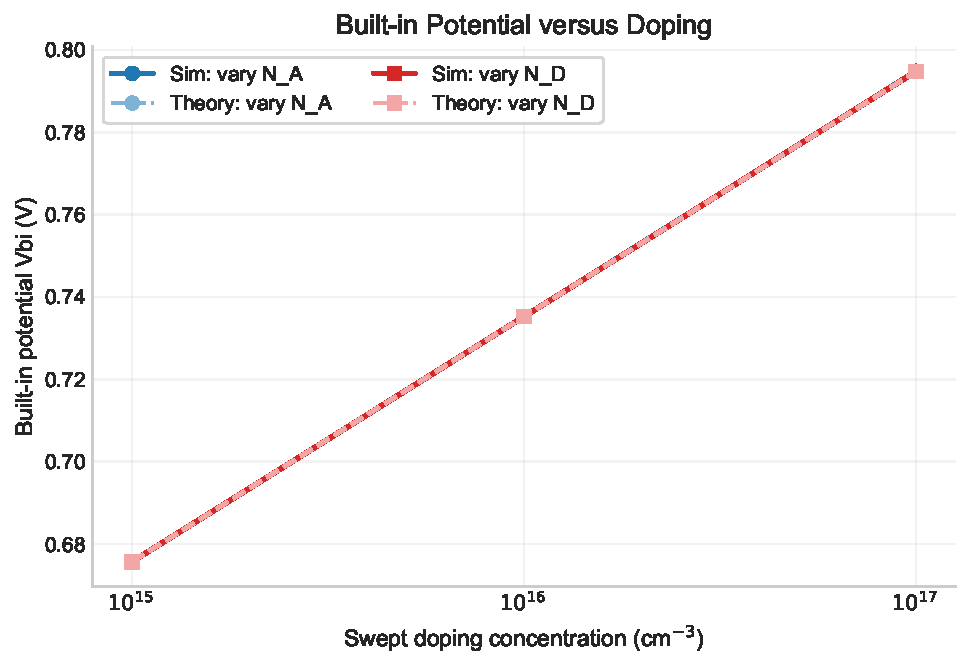
\includegraphics[width=\linewidth]{fig3_vbi_vs_doping.pdf}
        \caption{$\vbi$ vs doping.}
    \end{subfigure}
    \hfill
    \begin{subfigure}{0.48\textwidth}
        \centering
        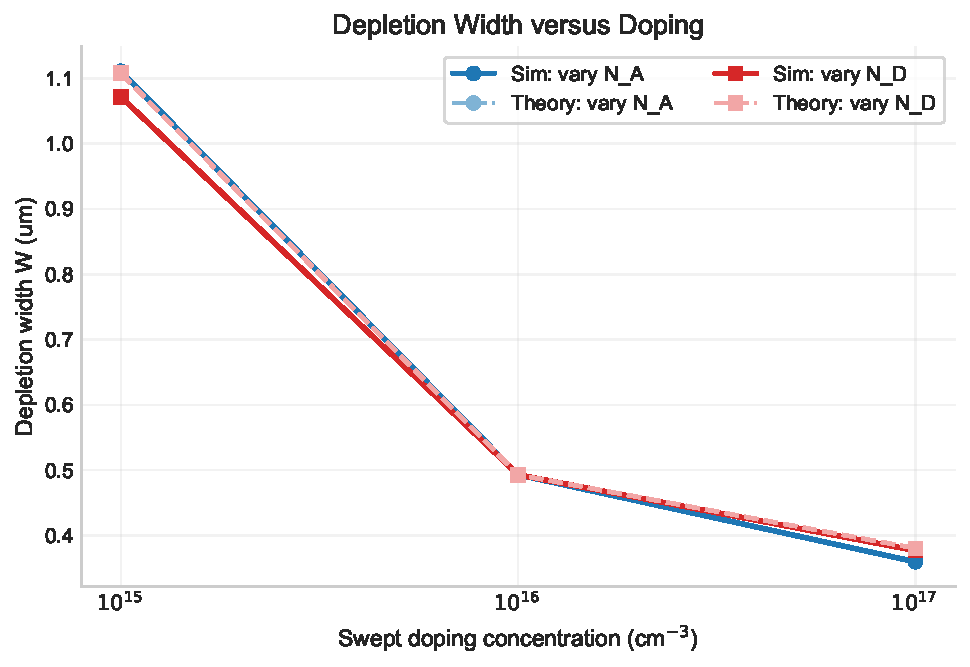
\includegraphics[width=\linewidth]{fig4_w_vs_doping.pdf}
        \caption{$W$ vs doping.}
    \end{subfigure}
    \caption{Dependence of built-in potential and depletion width on doping concentration.}
    \label{fig:vbi_w_doping}
\end{figure}

The $\vbi$ trend follows Equation~\ref{eq:vbi}: the built-in potential depends logarithmically on $\Na\Nd$. Therefore, even an order-of-magnitude doping change produces only a moderate voltage change. The depletion-width trend follows Equation~\ref{eq:depletion_width}. Although $\vbi$ increases slightly, the factor $(1/\Na+1/\Nd)$ decreases strongly as doping increases, so the depletion region becomes narrower.

\subsubsection{Saturation Current Density versus Doping}

Figure~\ref{fig:j0_vs_doping} shows the saturation current trend. The analytical model predicts that $\jzero$ decreases as doping increases because minority carrier concentrations scale as $n_i^2/N$. The simulation follows the same broad trend, but its absolute values remain higher than the ideal diffusion-current estimate.

\begin{figure}[htbp]
    \centering
    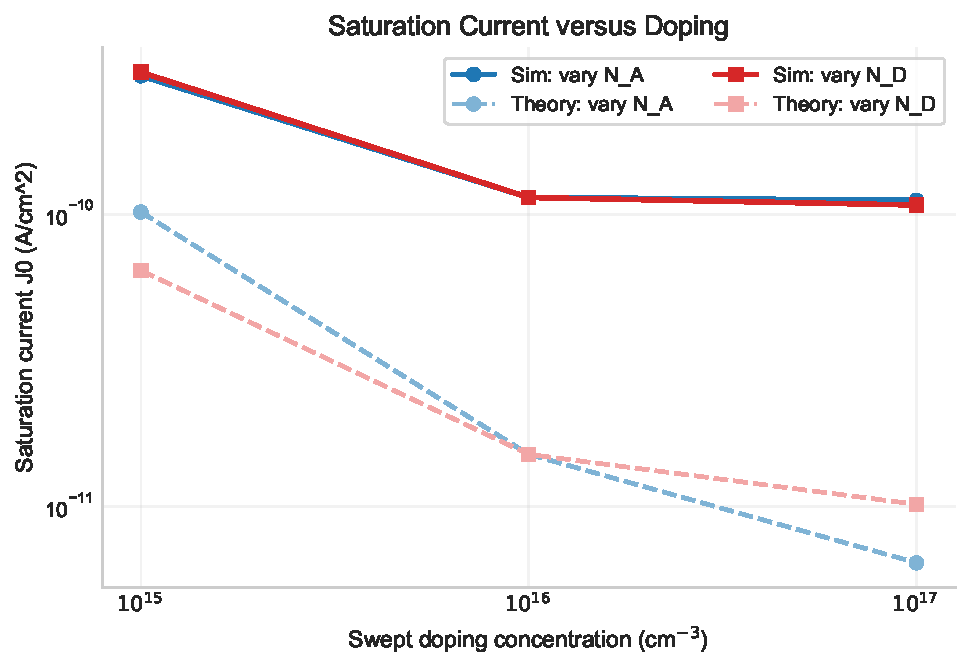
\includegraphics[width=0.80\linewidth]{fig5_j0_vs_doping.pdf}
    \caption{Saturation current density as a function of doping concentration.}
    \label{fig:j0_vs_doping}
\end{figure}

\subsubsection{Discussion of Doping Trends and Model Limitations}

The doping sweep confirms the expected semiconductor-device trends: higher doping increases $\vbi$, narrows $W$, and changes $\jzero$ through minority-carrier concentrations. The remaining numerical differences are expected because the analytical equations are simplified. They neglect depletion-region recombination, surface recombination, finite thickness, and the gradual field profile used in numerical depletion-width extraction.

Another important limitation is the constant-mobility assumption. The baseline simulation uses fixed values such as $\mu_n=\SI{1400}{cm^2/(V.s)}$ and $\mu_p=\SI{450}{cm^2/(V.s)}$. In real silicon, mobility decreases at high doping because ionized-impurity scattering becomes stronger. Therefore, high-doping deviations can partly arise from using constant mobility in the numerical model.

\subsection{Part 3: PIN Diode Basics}

\subsubsection{Intrinsic-layer Thickness Sweep}

Table~\ref{tab:pin_thickness_sweep} and Figure~\ref{fig:jsc_vs_di} show the PIN thickness sweep. Increasing the intrinsic-layer thickness increases the generation volume under the simplified uniform-generation model, so $|\jsc|$ increases. At the same time, $\voc$ decreases slightly and FF decreases, which is consistent with increased transport distance and series-resistance-like effects in thicker devices.

\begin{table}[htbp]
    \centering
    \caption{PIN diode simulation results for different intrinsic-layer thicknesses.}
    \label{tab:pin_thickness_sweep}
    \begin{tabular}{ccccc}
        \toprule
        $\di$ ($\um$) & $|\jsc|$ (\si{mA/cm^2}) & $\voc$ (V) & $W$ ($\um$) & FF \\
        \midrule
        0.5 & 39.3 & 0.5566 & 0.7908 & 0.7983 \\
        1.0 & 47.3 & 0.5545 & 1.2679 & 0.7849 \\
        2.0 & 63.2 & 0.5502 & 2.2679 & 0.7616 \\
        5.0 & 111.1 & 0.5435 & 5.2679 & 0.7222 \\
        \bottomrule
    \end{tabular}
\end{table}

\begin{figure}[htbp]
    \centering
    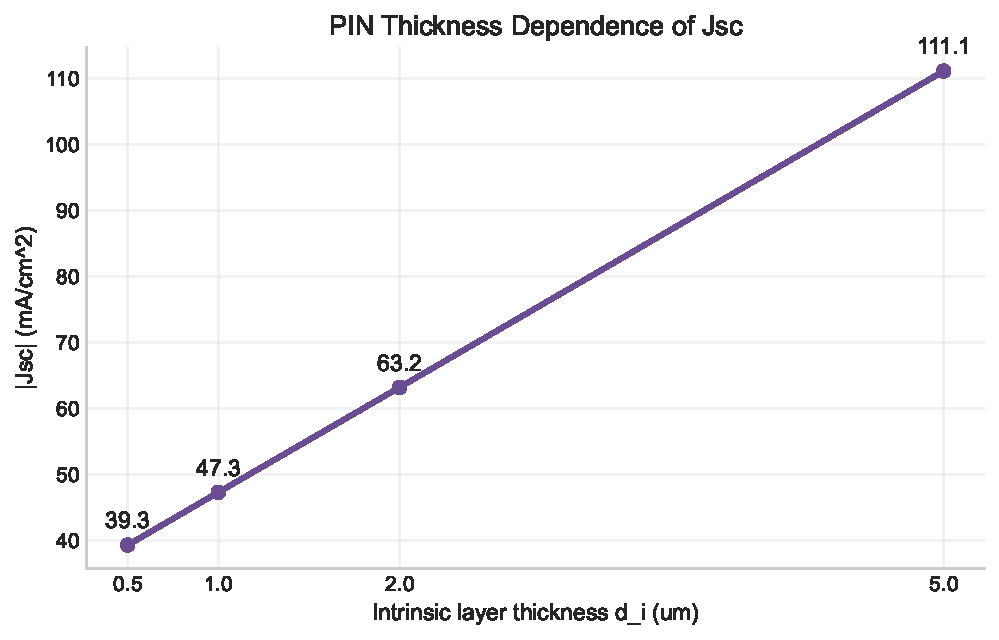
\includegraphics[width=0.78\linewidth]{fig6_jsc_vs_di.pdf}
    \caption{Short-circuit current density as a function of intrinsic-layer thickness.}
    \label{fig:jsc_vs_di}
\end{figure}

\subsubsection{PIN versus p--n Junction Comparison}

Task 3.2 compares the PIN diode with $\di=\SI{2}{\um}$ against a p--n junction with approximately the same total semiconductor thickness. The p--n comparison file uses a \SI{2}{\um} p-side and a \SI{2}{\um} n-side, while the PIN device uses \SI{1}{\um} p, \SI{2}{\um} intrinsic, and \SI{1}{\um} n regions. Both devices are therefore close to \SI{4}{\um} total thickness.

\begin{table}[htbp]
    \centering
    \caption{Task 3.2 comparison between same-thickness p--n and PIN devices.}
    \label{tab:pin_vs_pn}
    \begin{tabular}{lccc}
        \toprule
        Device & $|\jsc|$ (\si{mA/cm^2}) & $\voc$ (V) & $W$ ($\um$) \\
        \midrule
        p--n, same thickness & 61.44 & 0.5752 & 0.4756 \\
        PIN diode, $\di=\SI{2}{\um}$ & 63.24 & 0.5502 & 2.2679 \\
        \bottomrule
    \end{tabular}
\end{table}

\begin{figure}[htbp]
    \centering
    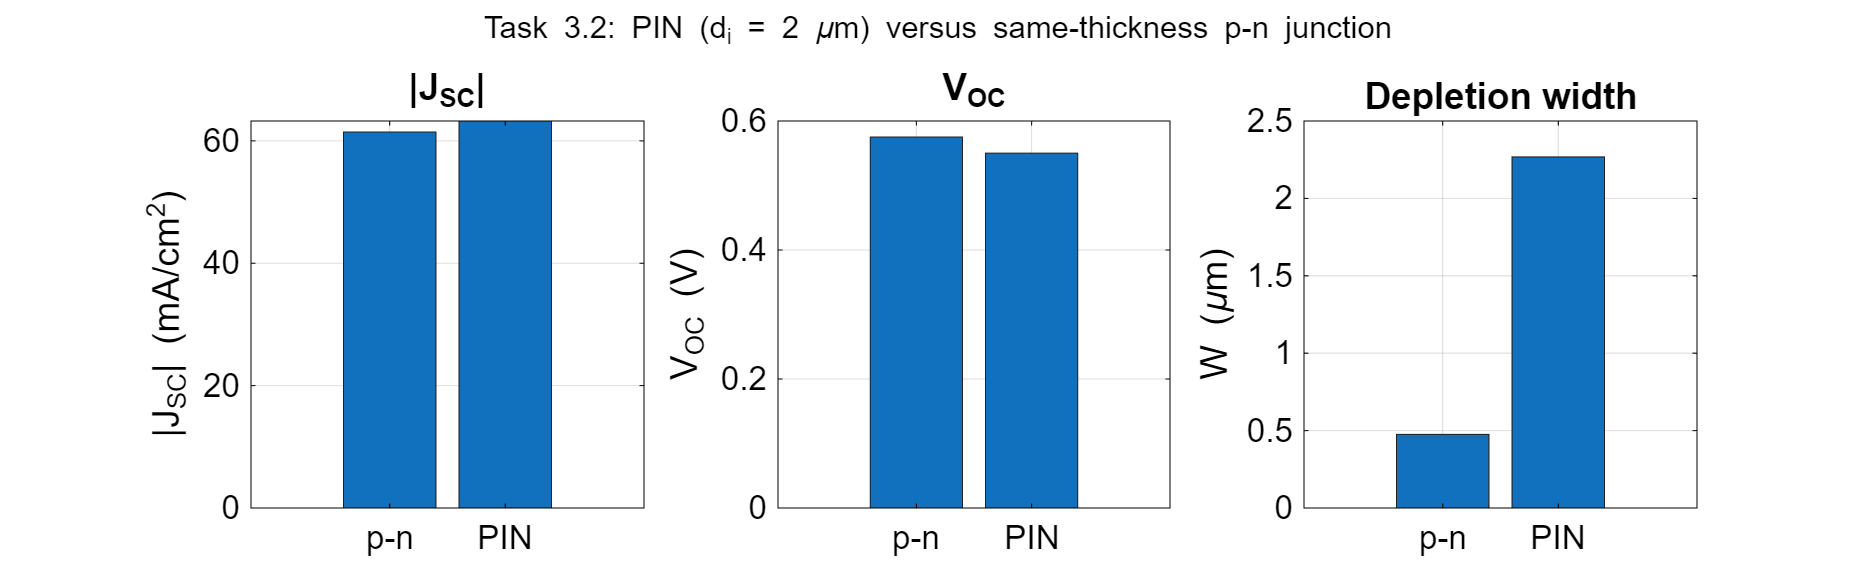
\includegraphics[width=0.82\linewidth]{task3_2_pin_vs_pn.png}
    \caption{Task 3.2 p--n and PIN comparison. With matched total thickness, the photocurrents are similar, while the PIN diode has a much wider depleted region.}
    \label{fig:pin_vs_pn}
\end{figure}

\subsubsection{Physical Interpretation: Drift Collection versus Diffusion Collection}

The PIN diode does not necessarily produce a larger $\jsc$ than a p--n diode under every simplified simulation setup. Its main advantage is the wide depleted intrinsic region. In a standard p--n junction, many photogenerated carriers are produced in quasi-neutral regions and must diffuse to the depletion edge before being swept out. Diffusion is slower and gives more opportunity for recombination.

In a PIN diode, the intrinsic layer is largely depleted, so a strong electric field extends across a much wider region. Photogenerated carriers in this region are collected primarily by drift, which is faster and more favorable for photodetection and high-frequency response. Driftfusion's discrete interface model is useful for this simulation because it smooths material and doping transitions over interface regions rather than forcing an abrupt jump at a single grid point, improving numerical stability while preserving the physical p/i/n structure.

\section{Conclusions}

Driftfusion successfully reproduces the expected p--n and PIN diode trends, but the deviations are the most informative part. The baseline p--n junction shows rectifying dark J--V behavior, and the illuminated simulation provides $\jsc$ and $\voc$ in a way consistent with diode theory. The extracted $\jzero$ is larger than the ideal analytical value because the analytical model omits finite-thickness effects, surface recombination, and SRH recombination.

The doping sweep agrees with analytical expectations: increasing doping raises $\vbi$ logarithmically and reduces $W$ because the space-charge region is more tightly confined. The $\jzero$ trend is governed by minority-carrier diffusion, while high-doping discrepancies can be explained partly by the constant-mobility assumption in the baseline model.

For the PIN diode, increasing the intrinsic-layer thickness increases the generation volume and widens the depletion region. The most important advantage of the PIN structure is not simply producing a larger current in all comparisons, but enabling drift-based carrier collection over a wider depleted region. Overall, the results show which device quantities are robustly described by simple analytical models and which require numerical drift-diffusion simulation to interpret correctly.

\section*{Individual Contribution Statement}
\addcontentsline{toc}{section}{Individual Contribution Statement}

\begin{itemize}[leftmargin=2em]
    \item \textbf{1A, Guo Wangyihan:} Built the baseline p--n junction simulation, generated the initial workspace, and provided baseline J--V and extraction data.
    \item \textbf{1B, Yang Chenhan:} Performed Part 2 doping sweeps, handled convergence issues at high doping, and extracted $\vbi$, $W$, and $\jzero$ from simulation.
    \item \textbf{1C, Jiang Ding:} Performed PIN diode thickness simulations and extracted $\jsc$, $\voc$, depletion width, and related raw data.
    \item \textbf{2A, Ma Yinfei:} Prepared analytical formulas for baseline comparison and analyzed surface-recombination and finite-thickness deviations.
    \item \textbf{2B, Wang Jiachang:} Prepared the theoretical interpretation of doping dependence and identified the constant-mobility limitation in the numerical model.
    \item \textbf{2C, Ji Yaofang:} Applied the discrete interface model to explain PIN behavior and formulated the physical explanation of drift versus diffusion collection.
    \item \textbf{3A, Chen Zhenbo:} Coordinated the project, integrated report sections, polished technical writing, and verified theoretical alignment.
    \item \textbf{3B, Shen Yishan:} Integrated the methodology section, including simulation protocols, parameter sweeps, and analytical-comparison workflow.
    \item \textbf{3C, Liu Yuxuan:} Standardized raw data into report-ready figures and formatted tables with consistent labels, units, and legends.
\end{itemize}

\appendix
\section{Code and Parameter Files}

\begin{table}[htbp]
    \centering
    \caption{Summary of code, data, and parameter files.}
    \label{tab:code_files}
    \begin{tabular}{llp{0.45\linewidth}}
        \toprule
        File & Used in & Description \\
        \midrule
        Part 1 CSV & Part 1 & Baseline p--n extraction results \\
        Part 2 CSV & Part 2 & Doping sweep results \\
        PIN CSV & Part 3 & PIN thickness sweep results \\
        Figure PDFs & Figures & Report-ready figures transferred from the presentation outputs \\
        \bottomrule
    \end{tabular}
\end{table}

\begin{thebibliography}{9}
\bibitem{streetman} Streetman, B. G., \& Banerjee, S. K. (2014). \textit{Solid State Electronic Devices} (7th ed.). Pearson.
\bibitem{driftfusion} Calado, P., Gelmetti, I., Hilton, B., Azzouzi, M., Nelson, J., \& Barnes, P. R. F. (2022). Driftfusion: an open source code for simulating ordered semiconductor devices with mixed ionic-electronic conducting materials in one dimension. \textit{Journal of Computational Electronics}, 21, 960--991.
\end{thebibliography}

\end{document}
